\begin{uebsp}
\begin{Exercise}
Berechnen Sie das Zeitsignal $x[n]$ für folgende Spektren:
\begin{enumerate}[a)]
    \item $\displaystyle X\left(e^{j\theta}\right) = \cos^2\theta$
    \item ~\\
        \begin{center}
        \begin{tikzpicture}
        \begin{axis}[
            domain=-2*pi:2*pi,
            axis x line=bottom, % no box around the plot, only x and y axis
            axis y line=left, % the * would suppress the arrow tips
            xlabel={$x$},
            ymax=1,
            legend pos=north east,
            samples=50,
            height=3cm,
            width=12cm,
            xtick={-6.2831, -3.1416, -2.09, 0, 2.09, 3.1416, 6.2831},
            xticklabels={$-2\pi$,$-\pi$,$-\theta_g$,$0$,$\theta_g$,$\pi$,$2\pi$},
            ytick={0,1},
            clip=false]
            \addplot[thin, smooth, blue,domain=0:2*pi/3] {1-3*x/(2*pi)};
            \addplot[thin, smooth, blue,domain=-2*pi/3:0] {3*x/(2*pi)+1};
            \addplot[thin, smooth, blue,domain=2*pi/3:4*pi/3] {0};
            \addplot[thin, smooth, blue,domain=-4*pi/3:-2*pi/3] {0};

            \addplot[thin, smooth, blue,domain=-2*pi:-4*pi/3] {-2-3*x/(2*pi)};
            \addplot[thin, smooth, blue,domain=4*pi/3:2*pi] {-2+3*x/(2*pi)};
            %\addlegendentry[align=left]{$\mathcal{N}(\muval, \sigmaval)$};
            %\draw [thick,dashed,black] (current axis.south-|{axis cs:\muval,0}) -- (current axis.north-|{axis cs:\muval,0}) node [above] {$\mu=\muval$};
        \end{axis}
        \end{tikzpicture}
        \end{center}
    \item ~\\
        \begin{center}
        \begin{tikzpicture}
        \begin{axis}[
            domain=-2*pi:2*pi,
            axis x line=bottom, % no box around the plot, only x and y axis
            axis y line=left, % the * would suppress the arrow tips
            xlabel={$x$},
            ymax=1,
            legend pos=north east,
            samples=50,
            height=3cm,
            width=12cm,
            xtick={-6.2831, -3.1416, 0, 3.1416, 6.2831},
            xticklabels={$-2\pi$,$-\pi$,$0$,$\pi$,$2\pi$},
            ytick={0,1},
            clip=false]
            \addplot[thin, smooth, blue,domain=0:pi] {1-x/(pi)};
            \addplot[thin, smooth, blue,domain=pi:2*pi] {2-x/(pi)};
            \addplot[thin, smooth, blue,domain=-pi:0] {-x/(pi)};
            \addplot[thin, smooth, blue,domain=-2*pi:-pi] {-1-x/(pi)};
            \addplot[mark=none, color=blue] coordinates {
                (-2*pi,1)
                (-2*pi,0)
            };
            \addplot[mark=none, color=blue] coordinates {
                (-pi,1)
                (-pi,0)
            };
            \addplot[mark=none, color=blue] coordinates {
                (0,1)
                (0,0)
            };
            \addplot[mark=none, color=blue] coordinates {
                (pi,1)
                (pi,0)
            };
            %\addlegendentry[align=left]{$\mathcal{N}(\muval, \sigmaval)$};
            %\draw [thick,dashed,black] (current axis.south-|{axis cs:\muval,0}) -- (current axis.north-|{axis cs:\muval,0}) node [above] {$\mu=\muval$};
        \end{axis}
        \end{tikzpicture}
        \end{center}
    \item $\displaystyle X\left(e^{j\theta}\right) =
        \frac{e^{-j\theta}}{1+\frac{1}{6}e^{-j\theta}-\frac{1}{6}e^{-j2\theta}}$
\end{enumerate}
\end{Exercise}
\begin{Answer}
\begin{enumerate}[a)]
    \item $X\left(e^{j\theta}\right) = \cos^2\theta$\\
        Als erstes versuchen wir, das $\cos^2$ zu eliminieren:
    \begin{uebsp_theory}
        Laut
        \href{http://de.wikipedia.org/wiki/Formelsammlung\_Trigonometrie\#Kosinus}{wikipedia}
        gilt:
        \[\cos^2 x = \frac{1}{2}\ \Big(1 + \cos (2x) \Big) \]
    \end{uebsp_theory}
    \[X\left(e^{j\theta}\right)=\cos^2\theta=\frac{1}{2}\left(\cos(2\theta)+1\right)\]
    \begin{definition}[Eulersche Formel]
        \[e^{j\varphi}=\cos(\varphi)+j\cdot\sin(\varphi)\]
        Bzw. 
        \[\sin x = \frac{e^{jx} - e^{-jx}}{2j}\;\;\;\text{ und
            }\;\;\;\cos x = \frac{e^{jx} + e^{-jx}}{2}\]
    \end{definition}

    \[X\left(e^{j\theta}\right)=\frac{1}{2}\left(\cos(2\theta)+1\right)=\frac{1}{2}\left(\frac{e^{j2\theta}
    + e^{-j2\theta}}{2}+1\right)\]

    \begin{uebsp_theory}
        Aus der Formelsammlung (Fouriertransformationspaare) folgt:
        \[\delta[n-N_0]\;\;\multimapdotbothA\;\;e^{-j\theta N_0}\]
    \end{uebsp_theory}

    \begin{definition}[Linearitätseigenschaft der Fouriertransformation]
        \[a_1x_1[n]+a_2x_2[n]\multimapdotbothA
        a_1X_1(e^{j\theta})+a_2X_2(e^{j\theta})\]
    \end{definition}

    Somit versuchen wir nun $X\left(e^{j\theta}\right)$ als Summe (denn es gilt ja
    auch die Linearitätseigenschaft) von
    $e^\text{irgendwas}$ darzustellen:

    \[X\left(e^{j\theta}\right)=\frac{1}{2}\left(\frac{e^{j2\theta}+e^{-j2\theta}}{2}+1\right)=\underbrace{e^{j2\theta}}_{\multimapdotbothB\;\;\delta[n+2]}\frac{1}{4}+\underbrace{e^{-j2\theta}}_{\multimapdotbothB\;\;\delta[n-2]}\frac{1}{4}+\underbrace{e^{0}}_{\multimapdotbothB\;\;\delta[n-0]}\frac{1}{2}\]
    \[X\left(e^{j\theta}\right)={e^{j2\theta}}\frac{1}{4}+{e^{-j2\theta}}\frac{1}{4}+{e^{0}}\frac{1}{2}\multimapdotbothB
    \frac{\delta[n+2]}{4}+\frac{\delta[n-2]}{4}+\frac{\delta[0]}{2}=x[n]\]

    \item ~\\
        \begin{center}
        \begin{tikzpicture}
        \begin{axis}[
            domain=-2*pi:2*pi,
            axis x line=bottom, % no box around the plot, only x and y axis
            axis y line=left, % the * would suppress the arrow tips
            xlabel={$x$},
            ymax=1,
            legend pos=north east,
            samples=50,
            height=3cm,
            width=12cm,
            ytick={0,1},
            xtick={-6.2831, -3.1416, -2.09, 0, 2.09, 3.1416, 6.2831},
            xticklabels={$-2\pi$,$-\pi$,$-\theta_g$,$0$,$\theta_g$,$\pi$,$2\pi$},
            clip=false]
            \addplot[thin, smooth, blue,domain=0:2*pi/3] {1-3*x/(2*pi)};
            \addplot[thin, smooth, blue,domain=-2*pi/3:0] {3*x/(2*pi)+1};
            \addplot[thin, smooth, blue,domain=2*pi/3:4*pi/3] {0};
            \addplot[thin, smooth, blue,domain=-4*pi/3:-2*pi/3] {0};

            \addplot[thin, smooth, blue,domain=-2*pi:-4*pi/3] {-2-3*x/(2*pi)};
            \addplot[thin, smooth, blue,domain=4*pi/3:2*pi] {-2+3*x/(2*pi)};
            %\addlegendentry[align=left]{$\mathcal{N}(\muval, \sigmaval)$};
            %\draw [thick,dashed,black] (current axis.south-|{axis cs:\muval,0}) -- (current axis.north-|{axis cs:\muval,0}) node [above] {$\mu=\muval$};
        \end{axis}
        \end{tikzpicture}
        \end{center}

        Beim Lösen der Aufgabe hilft die Faltung:\\
        \raisebox{-.5\height}{
        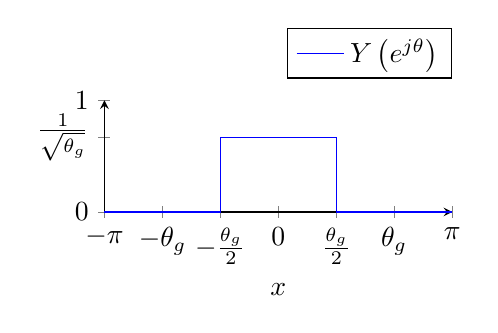
\begin{tikzpicture}
        \begin{axis}[
            domain=-pi:pi,
            axis x line=bottom, % no box around the plot, only x and y axis
            axis y line=left, % the * would suppress the arrow tips
            xlabel={$x$},
            ymax=1,
            legend style={at={(1,1.65), anchor=north west}},
            samples=50,
            height=3cm,
            width=6cm,
            xtick={-6.2831, -3.1416, -2.09, -1.05, 0, 1.05, 2.09, 3.1416, 6.2831},
            xticklabels={$-2\pi$,$-\pi$,$-\theta_g$,$-\frac{\theta_g}{2}$,$0$,$\frac{\theta_g}{2}$,$\theta_g$,$\pi$,$2\pi$},
            ytick={0,0.667,1},
            yticklabels={0,$\frac{1}{\sqrt{\theta_g}}$,1},
            clip=false]
            \addplot[mark=none, color=blue] coordinates {
                (-pi,0)
                (-pi/3,0)
                (-pi/3,2/3)
                (pi/3,2/3)
                (pi/3,0)
                (pi,0)
            };
            \addlegendentry[align=left]{$Y\left(e^{j\theta}\right)$};
        \end{axis}a
        \end{tikzpicture}}
        \raisebox{-.5\height}{$\xRightarrow{gefaltet}$}
        \raisebox{-.5\height}{
        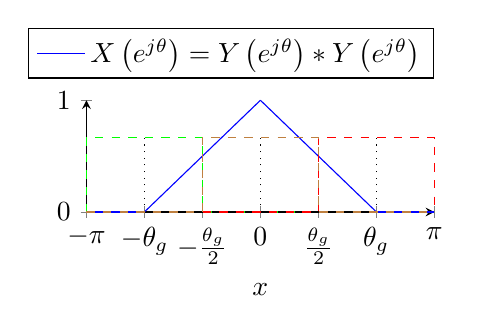
\begin{tikzpicture}
        \begin{axis}[
            domain=-pi:pi,
            axis x line=bottom, % no box around the plot, only x and y axis
            axis y line=left, % the * would suppress the arrow tips
            xlabel={$x$},
            ymax=1,
            legend style={at={(1,1.65), anchor=north west}},
            samples=50,
            height=3cm,
            width=6cm,
            xtick={-6.2831, -3.1416, -2.09, -1.05, 0, 1.05, 2.09, 3.1416, 6.2831},
            xticklabels={$-2\pi$,$-\pi$,$-\theta_g$,$-\frac{\theta_g}{2}$,$0$,$\frac{\theta_g}{2}$,$\theta_g$,$\pi$,$2\pi$},
            ytick={0,1},
            clip=false]
            \addplot[thin, smooth, blue,domain=0:2*pi/3] {1-3*x/(2*pi)};
            \addlegendentry[align=left]{$X\left(e^{j\theta}\right)=Y\left(e^{j\theta}\right)*Y\left(e^{j\theta}\right)$};
            \addplot[thin, smooth, blue,domain=-2*pi/3:0] {3*x/(2*pi)+1};
            \addplot[thin, smooth, blue,domain=2*pi/3:pi] {0};
            \addplot[thin, smooth, blue,domain=-pi:-2*pi/3] {0};

            \addplot[dotted, mark=none, color=black] coordinates {
                (0,0)
                (0,2/3)
            };
            \addplot[dotted, mark=none, color=black] coordinates {
                (-2*pi/3,0)
                (-2*pi/3,2/3)
            };
            \addplot[dotted, mark=none, color=black] coordinates {
                (2*pi/3,0)
                (2*pi/3,2/3)
            };

            \addplot[dashed,mark=none, color=green] coordinates {
                (-pi,0)
                (-pi,2/3)
                (-pi/3,2/3)
                (-pi/3,0)
                (pi,0)
            };
            \addplot[dashed,mark=none, color=red] coordinates {
                (-pi,0)
                (pi/3,0)
                (pi/3,2/3)
                (pi,2/3)
                (pi,0)
            };
            \addplot[dashed,mark=none, color=brown] coordinates {
                (-pi,0)
                (-pi/3,0)
                (-pi/3,2/3)
                (pi/3,2/3)
                (pi/3,0)
                (pi,0)
            };
        \end{axis}
        \end{tikzpicture}}

        Wenn 
        \[Y\left(e^{j\theta}\right)=\frac{1}{\sqrt{\theta_g}}
        \begin{cases}
            1& 0\leq|\theta|\leq\frac{\theta_g}{2}\\
            0& \frac{\theta_g}{2}<|\theta|<\pi\\
        \end{cases}\]
        dann ist die Faltung des Signals mit sich selbst ($\forall \theta_g<\pi$)
        \[X\left(e^{j\theta}\right)=Y\left(e^{j\theta}\right)*Y\left(e^{j\theta}\right)\]
        
        Nun haben wir das Signal und wir müssen es nur noch umtransformieren, um das Zeitsignal zu erhalten:
            \begin{definition}[Linearitätseigenschaft der Fouriertransformation]
                \[a_1x_1[n]+a_2x_2[n]\multimapdotbothA
                a_1X_1(e^{j\theta})+a_2X_2(e^{j\theta})\]
            \end{definition}

        \begin{uebsp_theory}
            Aus der Formelsammlung (Fouriertransformationspaare) folgt:
            \[\frac{\sin\alpha n}{\pi
                n},\;\;0<\alpha<\pi\;\;\;\multimapdotbothA\;\;\;X\left(e^{j\theta}\right)=
            \begin{cases}
                1& 0\leq|\theta|\leq\alpha\\
                0& \alpha<|\theta|<\pi\\
            \end{cases}\]
        \end{uebsp_theory}
        Somit können wir $Y\left(e^{j\theta}\right)\;\;\multimapdotbothB\;\;y[n]$ berechnen:
            \[Y\left(e^{j\theta}\right)=\frac{1}{\sqrt{\theta_g}}
        \begin{cases}
            1& 0\leq|\theta|\leq\frac{\theta_g}{2}\\
            0& \frac{\theta_g}{2}<|\theta|<\pi\\
    \end{cases}\;\;\;\multimapdotbothB\;\;\;\frac{1}{\sqrt{\theta_g}}\frac{\sin\frac{\theta_g}{2}}{\pi
n}=y[n]\]

        \begin{uebsp_theory}
                Aus der Formelsammlung (Fouriertransformation zeitdiskreter
                Signale) folgt:
                \[x[n]y[n]\;\;\;\multimapdotbothA\;\;\;\frac{1}{2\pi}\left(X\left(e^{j\theta}\right)*Y\left(e^{j\theta}\right)\right)\]
        \end{uebsp_theory}
        Somit können wir
        $X\left(e^{j\theta}\right)\;\;\;\multimapdotbothB\;\;\;x[n]$ berechnen:
        \[X\left(e^{j\theta}\right)=\frac{1}{2\pi}\left(Y\left(e^{j\theta}\right)*Y\left(e^{j\theta}\right)\right)\;\;\;\multimapdotbothB\;\;\;y[n]y[n]=\frac{x[n]}{2\pi}\]
        \[\;\;\Rightarrow\;\;
        2\pi\cdot
    X\left(e^{j\theta}\right)=\left(Y\left(e^{j\theta}\right)*Y\left(e^{j\theta}\right)\right)\;\;\;\multimapdotbothB\;\;\;2\pi\left(y[n]y[n]\right)=2\pi\left(y^2[n]\right)=x[n]\]
        \[\;\;\Rightarrow\;\;x[n]=2\pi\cdot
        \left(\frac{1}{\sqrt{\theta_g}}\frac{\sin\frac{\theta_g}{2}}{\pi
    n}\right)^2=\frac{2\cancel\pi\sin^2\frac{\theta_g}{2}}{\theta_g\cdot\pi^{\cancel{2}}n^2}
        =\frac{2\sin^2\frac{\theta_g}{2}}{\theta_g\cdot\pi n^2}\]

    \item ~\\
        \begin{center}
        \begin{tikzpicture}
        \begin{axis}[
            domain=-2*pi:2*pi,
            axis x line=bottom, % no box around the plot, only x and y axis
            axis y line=left, % the * would suppress the arrow tips
            xlabel={$x$},
            ymax=1,
            legend pos=north east,
            samples=50,
            height=3cm,
            width=12cm,
            xtick={-6.2831, -3.1416, 0, 3.1416, 6.2831},
            xticklabels={$-2\pi$,$-\pi$,$0$,$\pi$,$2\pi$},
            ytick={0,1},
            clip=false]
            \addplot[thin, smooth, blue,domain=0:pi] {1-x/(pi)};
            \addplot[thin, smooth, blue,domain=pi:2*pi] {2-x/(pi)};
            \addplot[thin, smooth, blue,domain=-pi:0] {-x/(pi)};
            \addplot[thin, smooth, blue,domain=-2*pi:-pi] {-1-x/(pi)};
            \addplot[mark=none, color=blue] coordinates {
                (-2*pi,1)
                (-2*pi,0)
            };
            \addplot[mark=none, color=blue] coordinates {
                (-pi,1)
                (-pi,0)
            };
            \addplot[mark=none, color=blue] coordinates {
                (0,1)
                (0,0)
            };
            \addplot[mark=none, color=blue] coordinates {
                (pi,1)
                (pi,0)
            };
            %\addlegendentry[align=left]{$\mathcal{N}(\muval, \sigmaval)$};
            %\draw [thick,dashed,black] (current axis.south-|{axis cs:\muval,0}) -- (current axis.north-|{axis cs:\muval,0}) node [above] {$\mu=\muval$};
        \end{axis}
        \end{tikzpicture}
        \end{center}

        Aufteilung von $X$ in $X_{pos}$ und $X_{neg}$:
        \[X\left(e^{j\theta}\right)=X_{pos}\left(e^{j\theta}\right)+X_{neg}\left(e^{j\theta}\right)\]
        \[X_{pos}=\frac{1}{2\pi}\int_{0}^{\pi}\left(1-\frac{\theta}{n}\right)e^{j\theta
        n} d\theta\]
        lt. Tutor soll das partiell integriert dann das folgende ergeben:

        \[\frac{1+jn\pi}{2\pi^2n^2}-\frac{(-1)^n}{2\pi^2n^2}\]

        Für die Berechnung von $X_{neg}$ reicht die Verschiebung im
        Frequenzbereich:
    \[X_{neg}[n]=X_{pos}(\theta+\pi)\;\;\Rightarrow\;\;x[n]=x_{pos}[n]+x_{neg}[n]=
        \begin{cases}x[n]=-\frac{1+(-1)^n}{j2\pi n}& \text{für } n\neq 0\\
        x[0]=\frac{1}{2} & \text{sonst}
    \end{cases}\]

    \attention{Bitte frage mich nie wie das genau gerechnet werden muss, denn ich
    weiß es nicht!!! (Aber scheinbar kommt sowas eh nicht zum Test)}
    \item $\displaystyle X\left(e^{j\theta}\right) =
        \frac{e^{-j\theta}}{1+\frac{1}{6}e^{-j\theta}-\frac{1}{6}e^{-j2\theta}}$

        Bei diesem Beispiel suchen wir ein Transformationspaar, das ähnlich, wie
        die Angabe aussieht:
        \begin{uebsp_theory}
            Aus der Formelsammlung (Fouriertransformationspaare) folgt:
            \[a^n\sigma[n],\;\;|a|<1\;\;\multimapdotbothA\;\;\frac{1}{1-ae^{-j\theta}}\]
        \end{uebsp_theory}
        Nun gilt es, unsere Formel so umzuformen, um dieses Transformationspaar
        verwenden zu können:

        \[X\left(e^{j\theta}\right) =
        \frac{e^{-j\theta}}{1+\frac{1}{6}e^{-j\theta}-\frac{1}{6}e^{-j2\theta}}\;\;\Rightarrow\;\;\fbox{Substituiere:
    $e^{-j\theta}=u$}\;\;\Rightarrow\;\;X\left(u\right) =
        \frac{u}{-\frac{1}{6}u^2+\frac{1}{6}u+1}\]

        \begin{definition}[Quadratische Lösungsformel]
            \[x_{1,2}=\frac{-b\pm\sqrt{b^2-4ac}}{2a}\]
        \end{definition}

        Bestimmen der Nullstellen, mittels der Quadratischen Lösungsformel:
        \begin{eqnarray*}
            u_{1,2}&=&\frac{-\frac{1}{6}\pm\sqrt{\left(\frac{1}{6}\right)^2+
                4\cdot\frac{1}{6}\cdot 1}}{-2\frac{1}{6}}
            =\frac{-\frac{1}{6}\pm\sqrt{\frac{1}{36}+
                \frac{4}{6}}}{-\frac{1}{3}}
            =\frac{-\frac{1}{6}\pm\sqrt{\frac{1}{36}+
                \frac{24}{36}}}{-\frac{1}{3}}
            =\frac{-\frac{1}{6}\pm\sqrt{\frac{25}{36}}}{-\frac{1}{3}}\\
            u_{1,2}&=&=\frac{-\frac{1}{6}\pm\frac{5}{6}}{-\frac{1}{3}}
            =\frac{\frac{1}{6}\mp\frac{5}{6}}{\frac{1}{3}}
            =3\left(\frac{1}{6}\mp\frac{5}{6}\right)
        \end{eqnarray*}
        \[u_1=3\frac{-4}{6}=\cancel3\frac{-2}{\cancel3}=-2\;\;\text{ und
        }\;\;u_2=3\frac{\cancel 6}{\cancel 6}=3\]

        Nun können wir uns die Faktoren ausdrücken, indem wir in $(u-u_1)$, bzw.
        $(u-u_2)$ einsetzen: 
        \[-\frac{1}{6}u^2+\frac{1}{6}u+1=(u+2)(u-3)x\]
        Berechnen des Korrekturfaktors $x$:
        \[-\frac{1}{6}u^2+\frac{1}{6}u+1=(u+2)(u-3)x\;\;\Rightarrow\;\;
            \frac{1}{6}\left(-u^2+u+6\right)=\left(u^2-3u+2u-6\right)x\]
            \[-\frac{1}{6}\cancel{\left(u^2-u-6\right)}=\cancel{\left(u^2-u-6\right)}x\;\;\Rightarrow\;\;x=-\frac{1}{6}\]

        \attention{Die Berechnung des Korrekturfaktors ist unbedingt notwendig,
            denn die Beziehung $a\cdot x^2+b\cdot x+c=(x-d)(x-e)$ gilt nur, wenn
        der Faktor $a=1$.}

        Jetzt können wir endlich die neue Form für $X(u)$ darstellen:
        \[X\left(u\right) =
        \frac{u}{-\frac{1}{6}u^2+\frac{1}{6}u+1}=\frac{u}{(u+2)(u-3)\left(-\frac{1}{6}\right)}=\frac{u}{(u+2)(u-3)}\left(-6\right)\]

        Nun müssen wir mittels Partialbruchzerlegung eine Summe erzeugen:
        \[\frac{u}{(u+2)(u-3)}\cancel{\left(-6\right)}=\left(\frac{A}{u+2}+\frac{B}{u-3}\right)\cancel{\left(-6\right)}\]
        \begin{eqnarray*}
            \frac{u}{(u+2)(u-3)}&=&\frac{A}{u+2}+\frac{B}{u-3}\\
            u&=&\frac{A\cancel{(u+2)}(u-3)}{\cancel{u+2}}+\frac{B(u+2)(\cancel{u-3})}{\cancel{u-3}}\\
            u&=&A(u-3)+B(u+2)
        \end{eqnarray*}
        Einsetzen der Nullstelle $u_1=-2$:
        \[u=A(u-3)+B(u+2)\;\;\Rightarrow\;\;-2=A(-2-3)+B(-2+2)\;\;\Rightarrow\;\;-2=A\cdot(-5)+B\cdot0\;\;\Rightarrow\;\;A=\frac{2}{5}\]
        Einsetzen der Nullstelle $u_2=3$:
        \[u=A(u-3)+B(u+2)\;\;\Rightarrow\;\;3=A(3-3)+B(3+2)\;\;\Rightarrow\;\;3=B\cdot
        5\;\;\Rightarrow\;\;B=\frac{3}{5}\]

        Einsetzen für $A$ und $B$ und dann besitzen wir endlich eine Äquivalente Summendarstellung unseres
        $X(u)$:
        \begin{eqnarray*}
            X\left(u\right) &=&
                \frac{u}{-\frac{1}{6}u^2+\frac{1}{6}u+1}=\frac{u}{(u+2)(u-3)}\left(-6\right)
            =\left(\frac{\frac{2}{5}}{u+2}+\frac{\frac{3}{5}}{u-3}\right)\left(-6\right)\\
            X\left(u\right) &=&
            \left(\frac{2}{u+2}+\frac{3}{u-3}\right)\left(-\frac{6}{5}\right)
            =\left(-\frac{6}{5}\right)\left(\frac{1}{\frac{u}{2}+1}+\frac{1}{\frac{u}{3}-1}\right)
    \end{eqnarray*}
        \begin{uebsp_theory}
            Aus der Formelsammlung (Fouriertransformationspaare) folgt:
            \[a^n\sigma[n],\;\;|a|<1\;\;\multimapdotbothA\;\;\frac{1}{1-ae^{-j\theta}}\]
        \end{uebsp_theory}
    Rücksubstituieren: $u=e^{-j\theta}$
        \begin{eqnarray*}
            X\left(e^{-j\theta}\right) &=&
            \left(-\frac{6}{5}\right)\left(\frac{1}{\frac{e^{-j\theta}}{2}+1}+\frac{1}{\frac{e^{-j\theta}}{3}-1}\right)=\frac{6}{5}\left(\frac{1}{\frac{-e^{-j\theta}}{2}-1}+\frac{1}{\frac{-e^{-j\theta}}{3}+1}\right)\\
            X\left(e^{-j\theta}\right) &=&
            \frac{6}{5}\left(\frac{1}{-1-\frac{1}{2}e^{-j\theta}}+\frac{1}{1-\frac{1}{3}e^{-j\theta}}\right)
            = 
            \frac{6}{5}\left(-\frac{1}{1+\frac{1}{2}e^{-j\theta}}+\frac{1}{1-\frac{1}{3}e^{-j\theta}}\right)\\
            X\left(e^{-j\theta}\right) &=&
            \frac{6}{5}\left(-\frac{1}{1-\left(-\frac{1}{2}\right)e^{-j\theta}}+\frac{1}{1-\frac{1}{3}e^{-j\theta}}\right)\;\;\multimapdotbothB\;\;
            \frac{6}{5}\left(-\left(-\frac{1}{2}\right)^n\sigma[n]+\left(\frac{1}{3}\right)^n\sigma[n]\right)
            = x[n]
    \end{eqnarray*}

    \[x[n]=\frac{6}{5}\left(\left(\frac{1}{3}\right)^n-\left(-\frac{1}{2}\right)^n\right)\sigma[n]\]
\end{enumerate}
\end{Answer}
\end{uebsp}

